%%%%%%%%%%%%%%%%%%%%%%%%%%%%%%%%% Search Strategy : Performance Estimation Strategy %%%%%%%%%%%%%%%%%%
\begin{frame}{Annexe \ref{ap:performance_estimation} : Stratégie d'Evaluation de Solutions}
    \label{ap:performance_estimation}
    \begin{block}{Implémentation}
        \begin{itemize}
            \item Fine Tuning
            \begin{itemize}
                \item Modèle : LlaMa-3.2-1B
                \item Jeu de données d'entrainement : Alpaca
                \item LitGPT framework : basé sur Pytorch, facilite le Fine Tuning de LLM
            \end{itemize}
            \item Evaluation
            \begin{itemize}
                \item librairie lm\_eval : standard pour l'évaluation de LLM
                \item Evaluation par la précision sur des jeu de données Benchmark : Hellaswag et MMLU
            \end{itemize}
        \end{itemize}

        
    \end{block}

\end{frame}

%%%%%%%%%%%%%%%%%%%%%%%%%%%%%%%%% Transformer %%%%%%%%%%%%%%%%%%
\begin{frame}{Annexe \ref{ap:llm_architecture} : Transformer architecture}
    \label{ap:llm_architecture}
    \begin{figure}
        \centering
        \begin{tikzpicture}[node distance=0.8cm]


    \tikzstyle{norm} = [rectangle, rounded corners, minimum width=1cm ,text centered, draw=black, fill=red!30]
    \tikzstyle{mha} = [rectangle,rounded corners, minimum width=2cm , text centered, draw=black, fill=orange!30]
    \tikzstyle{feed} = [rectangle, rounded corners, minimum width=1cm ,text centered, draw=black, fill=blue!40]
    \tikzstyle{embed} = [rectangle, rounded corners, minimum width=1cm ,text centered, draw=black, fill=pink!30]
    \tikzstyle{encoding} = [rectangle, rounded corners, minimum width=1cm ,text centered, draw=black, fill=pink!40]
    \tikzstyle{linear} = [rectangle, rounded corners, minimum width=1cm ,text centered, draw=black, fill=blue!20]
    \tikzstyle{softmax} = [rectangle, rounded corners, minimum width=1cm ,text centered, draw=black, fill=green!20]
    
    
    \tikzstyle{arrow} = [thick,->,>=stealth]
    \tikzstyle{lightA} = [thick,dotted,->,>=stealth]
    
    \tikzstyle{sum} = [circle, draw, minimum size=0.5cm, node distance=1cm, inner sep=0pt]
    
    % Decoder node
    
    \node (norm3)[norm,yshift = -0.5cm]{Add \& Norm};
    \node (feed2)[feed,below of = norm3, yshift = 0.1cm]{Feed-Forward};
    
    \node (norm4)[norm,below of = feed2,yshift=0.1cm]{Add \& Norm};
    \node (mha2)[mha,below of = norm4, yshift = 0.1cm]{MHA};
    
    \node (norm5)[norm,below of = mha2,yshift=-0.5cm]{Add \& Norm};
    \node (mha3)[mha,below of = norm5]{Masked MHA};
    
    % Encoder node
    
    \node (norm1)[norm,left of = norm4, xshift=-3cm]{Add \& Norm};
    \node (feed1)[feed,below of = norm1]{Feed-Forward};
    
    \node (norm2)[norm,below of = feed1,yshift=-0.5cm]{Add \& Norm};
    \node (mha1)[mha,below of = norm2]{MHA};
    
    % Arrow inside encoder
    \node (enc_base)[below of = mha1]{};
    
    \draw[lightA] (enc_base.center) -- (mha1);
    \draw[lightA] (enc_base.center) -- ([xshift=-0.4cm, yshift = -0.4cm]mha1.south) -- ([xshift=-0.4cm]mha1.south);
    \draw[lightA] ([yshift = -0.3cm]enc_base.center) -- (enc_base.center) -- ([xshift=0.4cm, yshift = -0.4cm]mha1.south) -- ([xshift=0.4cm]mha1.south);
    
    \draw[lightA] ([yshift = -0.3cm]enc_base.center) -- ([yshift = -0.3cm,xshift = -1.3cm]enc_base.center) -- ([xshift = -1.3cm]norm2.center) -- (norm2.west);
    
    \draw [lightA] (mha1) -- (norm2); 
    \draw [lightA] (norm2) -- (feed1); 
    \draw [lightA] (feed1) -- (norm1); 
    
    \draw[lightA] ([yshift = 0.6cm]norm2.center) -- ([xshift = -1.3cm,yshift = 0.6cm]norm2.center) -- ([xshift = -1.3cm]norm1.center) -- (norm1.west);
    
    \node(enc_fit)[draw, thick, dashed, rounded corners, fit=(norm1)(feed1)(norm2)(enc_base), inner sep=0.4cm, label=left:{N $\times$ }] {};
    
    % Arrow inside decoder
    \node (dec_base)[below of = mha3]{};
    
    \draw[lightA] (dec_base.center) -- (mha3);
    \draw[lightA] (dec_base.center) -- ([xshift=-0.4cm, yshift = -0.4cm]mha3.south) -- ([xshift=-0.4cm]mha3.south);
    \draw[lightA] ([yshift = -0.3cm]dec_base.center) -- (dec_base.center) -- ([xshift=0.4cm, yshift = -0.4cm]mha3.south) -- ([xshift=0.4cm]mha3.south);
    
    \draw[lightA] ([yshift = -0.3cm]dec_base.center) -- ([yshift = -0.3cm,xshift = 1.3cm]dec_base.center) -- ([xshift = 1.3cm]norm5.center) -- (norm5.east);
    
    \draw [lightA] (mha3) -- (norm5); 
    
    \draw [lightA] (norm5) --([yshift = 0.4cm]norm5.center) -- ([yshift=-0.4cm,xshift=0.4cm]mha2.south) -- ([xshift=0.4cm]mha2.south); 
    
    \draw [lightA] (mha2) -- (norm4); 
    \draw [lightA] (norm4) -- (feed2); 
    \draw [lightA] (feed2) -- (norm3); 
    
    \draw[lightA] ([yshift = 0.4cm]norm5.center) -- ([xshift = 1.3cm,yshift = 0.4cm]norm5.center) -- ([xshift = 1.3cm]norm4.center) -- (norm4.east);
    \draw[lightA] ([yshift = 0.6cm]norm4.center) -- ([xshift = 1.3cm,yshift = 0.6cm]norm4.center) -- ([xshift = 1.3cm]norm3.center) -- (norm3.east);
    
    \node(dec_fit)[draw, thick, dashed, rounded corners, fit=(norm3)(dec_base), inner sep=0.2cm, label=right:{$\times$ N}] {};
    
    %arrow from encoder to decoder
    
    \draw[arrow] (norm1.north) -- ([yshift=0.4cm]enc_fit.north)
        -- ([yshift=0.4cm, xshift = 2cm]enc_fit.north)
        -- ([yshift=-2.2cm, xshift = 2cm]enc_fit.north)
         -- ([yshift=-2.2cm, xshift = 3.8cm]enc_fit.north)
         -- (mha2.south);
    \draw[arrow] ([yshift = -0.45cm, xshift = -0.4cm]mha2.south) -- ([xshift = -0.4cm]mha2.south);
    
    % encoder input
    \node (enc_plus) [sum, below of = enc_base,yshift=-0.1cm]{\Large $+$};
    \node (in_embed) [embed, below of = enc_plus,align=center, yshift = -0.2cm]{Input \\ Embedding};
    \node (encoding1) [encoding,left of = enc_plus, align = center, xshift = -1.5cm, yshift=-0.2cm]{Positional \\ Encoding};
    \node (input) [below of = in_embed, yshift = -0.3cm]{Input};
    
    % Decoder Input
    \node (dec_plus) [sum, below of = dec_base,yshift=-0.1cm]{\Large $+$};
    \node (out_embed) [embed, below of = dec_plus,align=center, yshift = -0.2cm]{Ouput \\ Embedding};
    \node (encoding2) [encoding,right of = dec_plus, align = center, xshift = 1.5cm, yshift=-0.2cm]{Positional \\ Encoding};
    \node (output) [below of = out_embed, yshift = -0.3cm, align = center]{Ouputs \\ (shifted right)};
    
    %outputs
    \node (linear) [linear, above of = norm3, yshift = -0.1cm]{Linear};
    \node (softmax) [softmax, above of = linear, yshift = -0.1cm]{Softmax};
    \node (out) [above of = softmax,align = center, yshift=-0.1cm]{Output};
    
    
    % I/O arrow
    \draw[arrow] (input) -- (in_embed);
    \draw[arrow] (in_embed) -- (enc_plus);
    
    
    \draw[arrow] (input.west) -- ([ yshift = -0.8cm]encoding1.south) -- (encoding1);
    \draw[arrow] (output.east) -- ([ yshift = -0.8cm]encoding2.south) -- (encoding2);
    
    
    \draw[arrow] (output) -- (out_embed);
    \draw[arrow] (out_embed) -- (dec_plus);
    \draw[arrow] (encoding1) -- (enc_plus);
    \draw[arrow] (encoding2) -- (dec_plus);
    \draw[arrow] (enc_plus) -- ([yshift = -0.3cm]enc_base.center);
    \draw[arrow] (dec_plus) -- ([yshift = -0.3cm]dec_base.center);
    \draw[arrow] (norm3.north) -- (linear);
    \draw[arrow] (linear) -- (softmax);
    \draw[arrow] (softmax) -- (out);
    \draw[arrow] (out.north) -- ([yshift = 0.2cm]out.north);
    
    % Encoder and Decoder Legend
    \node [left of = enc_base,xshift= -2cm, yshift = 1cm]{\textbf{Encoder}};
    \node [right of = dec_base,xshift= 2cm, yshift = 1cm]{\textbf{Decoder}};
    
    \end{tikzpicture}
        \caption{Illustration du mécanisme d'auto-attention : A droite le mécanisme complet, a gauche le \textit{Scaled Dot-product Attention}}
    \end{figure}
    
\end{frame}

%%%%%%%%%%%%%%%%%%%%%%%%%%%%%%%%% Multi-Head Attention %%%%%%%%%%%%%%%%%%
\begin{frame}{Annexe \ref{ap:mha} : Multi-Head Attention}
    \label{ap:mha}
    \begin{figure}
        \centering
        \begin{tikzpicture}[node distance=0.8cm]

\tikzstyle{matmul} = [rectangle,rounded corners, minimum width=2cm , text centered, draw=black, fill=purple!30]
\tikzstyle{softmax} = [rectangle,rounded corners, minimum width=2cm , text centered, draw=black, fill=green!30]
\tikzstyle{mask} = [rectangle,rounded corners, minimum width=2cm , text centered, draw=black, fill=pink!30]
\tikzstyle{sca} = [rectangle, rounded corners, minimum width=2cm ,text centered, draw=black, fill=yellow!30]
\tikzstyle{action} = [rectangle, rounded corners, minimum width=2cm ,text centered, draw=black, fill=red!30]
\tikzstyle{arrow} = [thick,->,>=stealth]

\tikzstyle{linear} = [rectangle, rounded corners, minimum width=1cm ,text centered, draw=black, fill=blue!30]
\tikzstyle{dot-prod} = [rectangle, rounded corners, minimum width=2cm,minimum height = 1cm ,text centered, draw=black, fill=purple!50]
\tikzstyle{concat} = [rectangle, rounded corners, minimum width=2cm ,text centered, draw=black, fill=yellow!50]



% Define nodes
\node (matmul1) [matmul]{Matmul};
\node (softmax)[softmax, below of = matmul1, xshift = -0.8cm]{Softmax};
\node (mask) [mask, below of=softmax]{Mask (opt.)};
\node (scale) [sca, below of=mask]{Scale};
\node (matmul2) [matmul, below of=scale]{Matmul};
\node (q) [below of=matmul2, xshift=-0.5cm]{Q};
\node (k) [below of=matmul2, xshift=0.5cm]{K};
\node (v) [below of=matmul2, xshift=1.5cm]{V};


% Draw arrows
\draw [arrow] (matmul1.north) -- ([yshift=0.5cm]matmul1.north);
\draw [arrow] (softmax.north) -- ([xshift=-0.8cm]matmul1.south);
\draw [arrow] (mask.north) -- (softmax.south);
\draw [arrow] (scale.north) -- (mask.south);
\draw [arrow] (matmul2.north) -- (scale.south);
\draw [arrow] (q.north) -- ([xshift=-0.5cm]matmul2.south);
\draw [arrow] (k.north) -- ([xshift=0.5cm]matmul2.south);
\draw [arrow] (v.north) -- ([xshift=0.7cm]matmul1.south);


% MHA 
\node (linear1) [linear, right of = matmul1, xshift = 5cm] {Linear};
\node (concat) [concat, below of = linear1] {Concat};
\node (dot-prod) [dot-prod, below of = concat,yshift= -0.4cm] {Scaled Dot-product Attention};
\node (linear2) [linear, below of = dot-prod, xshift = -1.5cm, yshift = -0.4cm] {Linear};
\node (linear3) [linear, below of = dot-prod, yshift = -0.4cm] {Linear};
\node (linear4) [linear, below of = dot-prod, xshift = 1.5cm, yshift = -0.4cm] {Linear};
\node (q2) [below of=linear2]{Q};
\node (k2) [below of=linear3]{K};
\node (v2) [below of=linear4]{V};

% MHA arrow
\draw [arrow] (q2) -- (linear2);
\draw [arrow] (k2) -- (linear3);
\draw [arrow] (v2) -- (linear4);
\draw [arrow] (linear2.north) -- ([xshift=-1.5cm]dot-prod.south);
\draw [arrow] (linear3.north) -- (dot-prod.south);
\draw [arrow] (linear4.north) -- ([xshift=1.5cm]dot-prod.south);
\draw [arrow] (dot-prod) -- (concat);
\draw [arrow] (concat) -- (linear1);
\draw [arrow] (linear1.north) -- ([yshift=0.5cm]linear1.north);

% MHA * h
\node[draw, thick, dashed, rounded corners, fit=(dot-prod), inner sep=0.1cm, label=right:{$\times$ h}] {};
\node[draw, thick, dashed, rounded corners, fit=(linear2)(linear3)(linear4), inner sep=0.1cm, label=right:{$\times$ h}] {};


% Title
\node (dot_t) [above of = matmul1,yshift=0.5cm] {\textbf{Scaled Dot-Product Attention}};
\node (mha) [above of = linear1,yshift=0.5cm] {\textbf{Multi-Head Attention}};



\end{tikzpicture}
        \caption{Illustration du mécanisme d'auto-attention : A droite le mécanisme complet, a gauche le \textit{Scaled Dot-product Attention}}
    \end{figure}
    
\end{frame}

%%%%%%%%%%%%%%%%%%%%%%%%%%%%%%%%% Low Rank Adaptation %%%%%%%%%%%%%%%%%%
\begin{frame}{Annexe \ref{ap:lora} : Low Rank Adaptation (LoRA)}
    \label{ap:lora}
    \begin{figure}
        \centering
        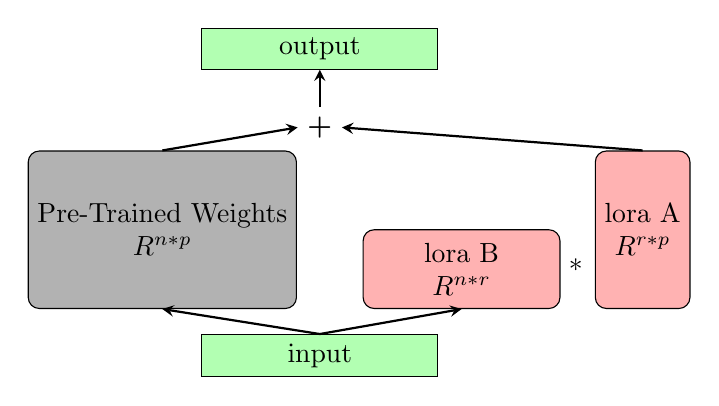
\begin{tikzpicture}[node distance=1.8cm]
    % Define block styles
    \tikzstyle{weights} = [rectangle,rounded corners, minimum width=2.5cm, minimum height=2cm, text centered, draw=black, fill=black!30]
    \tikzstyle{lora_a} = [rectangle,rounded corners, minimum width=1cm, minimum height=2cm, text centered, draw=black, fill=red!30]
    \tikzstyle{lora_b} = [rectangle,rounded corners, minimum width=2.5cm, minimum height=1cm, text centered, draw=black, fill=red!30]
    \tikzstyle{vector} = [rectangle, minimum width=3cm, minimum height=0.5cm, text centered, draw=black, fill=green!30]
    \tikzstyle{arrow} = [thick,->,>=stealth]
    
    % Define nodes
    \node (weights) [weights, align=center]{Pre-Trained Weights \\ $\mathbb{R}^{n*p}$};
    \node (lora_B) [lora_b, right of=weights,xshift=2cm,yshift=-0.5cm, align=center]{lora B\\ $\mathbb{R}^{n*r}$};
    \node (mul) [right of = lora_B,xshift=-0.35cm]{*};
    \node (lora_A) [lora_a, right of=lora_B,xshift=0.5cm,yshift=0.5cm, align=center]{lora A\\$\mathbb{R}^{r*p}$};
    \node (input) [vector,below of = weights, xshift = 2cm,yshift=+0.2cm]{input};
    \node (plus) [above of = weights, xshift = 2cm,yshift=-0.5cm]{\textbf{+}};
    \node (output) [vector,above of = plus,yshift=-0.8cm]{output};
    
    
    
    
    % Draw arrows
    \draw [arrow] (input.north) -- (weights.south);
    \draw [arrow] (input.north) -- (lora_B.south);
    \draw [arrow] (weights.north) -- (plus.west);
    \draw [arrow] (lora_A.north) -- (plus.east);
    \draw [arrow] (plus) -- (output);
    
    
    \end{tikzpicture}
        \caption{Illustration de l'application du Low Rank Adaptation (LoRA)}
    \end{figure}
    
\end{frame}


%%%%%%%%%%%%%%%%%%%%%%%%%%%%%%%%% BO results %%%%%%%%%%%%%%%%%%
\begin{frame}{Annexe \ref{ap:bo_results} : Résultats pour BO}
    \label{ap:bo_results}
    \begin{figure}
        \centering
        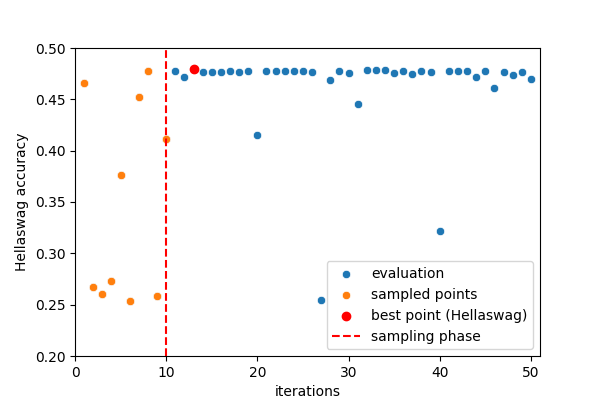
\includegraphics[height = 5cm]{assets/imgs/plots/bo/score_evolution.png}
        \caption{Evolution des score lors de l'expérience BO}
    \end{figure}
\end{frame}

%%%%%%%%%%%%%%%%%%%%%%%%%%%%%%%%% SOO results %%%%%%%%%%%%%%%%%%
\begin{frame}{Annexe \ref{ap:soo_results} : Résultats pour SOO}
    \label{ap:soo_results}
    \begin{figure}
        \centering
        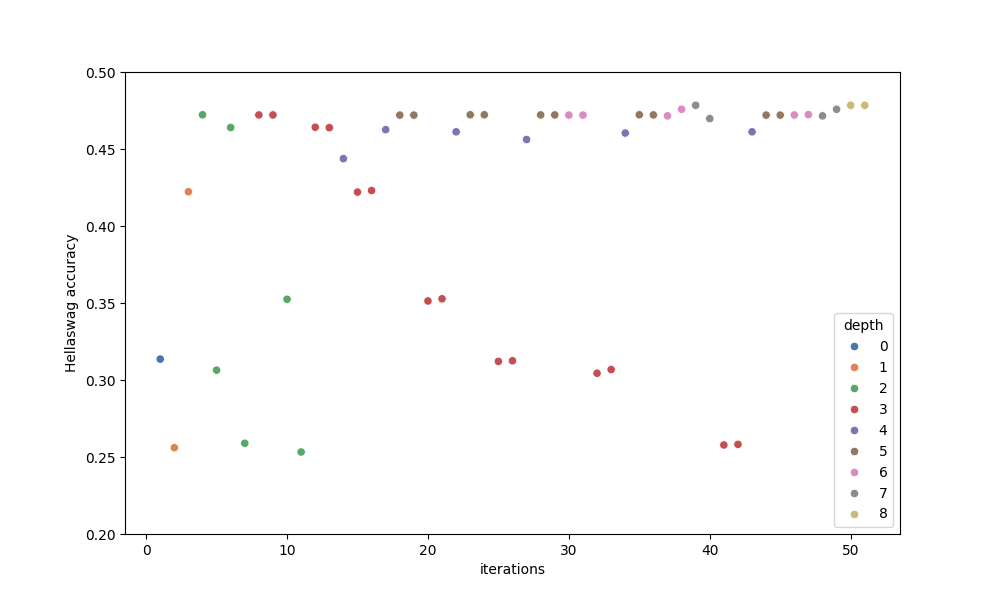
\includegraphics[height = 5cm]{assets/imgs/plots/soo/score_evolution.png}
        \caption{Evolution des score lors de l'expérience SOO}
    \end{figure} 
\end{frame}

%%%%%%%%%%%%%%%%%%%%%%%%%%%%%%%%% BaMSOO results %%%%%%%%%%%%%%%%%%
\begin{frame}{Annexe \ref{ap:bamsoo_results} : Résultats pour BaMSOO}
    \label{ap:bamsoo_results}
    \begin{figure}
        \centering
        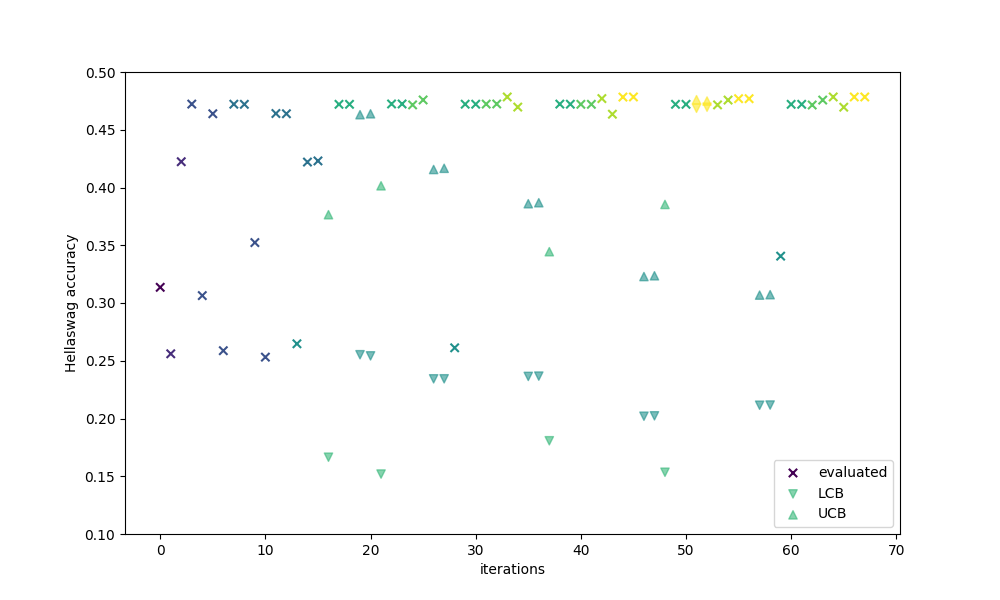
\includegraphics[height = 5cm]{assets/imgs/plots/bamsoo/score_evolution.png}
        \caption{Evolution des score lors de l'expérience BaMSOO}
    \end{figure} 
\end{frame}

%%%%%%%%%%%%%%%%%%%%%%%%%%%%%%%%% Beamer Template %%%%%%%%%%%%%%%%%%
\begin{frame}{Annexe \ref{ap:beamer_template} : Modèle Beamer UTT}
    \label{ap:beamer_template}
    \begin{figure}
        \centering
        
\includegraphics[width = 0.7\textwidth]{assets/annexes/beamer_gh_screenshot.png}
        \caption{Presentation du template beamer sur github : \href{https://github.com/Kiwy3/beamer_utt_template}{lien} }
    \end{figure} 
\end{frame}